% Author: Adolfo Centeno 
% Kubeet Corp
% www.kubeet.com

 
\documentclass{beamer}
\setbeamertemplate{navigation symbols}{}
\usepackage[utf8]{inputenc}
\usepackage{beamerthemeshadow}
\usepackage{listings}

\begin{document}
\title{Angular - Unit testing}  
\author{Adolfo Centeno}
\date{\today} 

\begin{frame}
\titlepage
\end{frame}

\begin{frame}\frametitle{Table of contents}\tableofcontents
\end{frame} 


\section{install Angular - Testing Intro - developer 3} 


\defverbatim[colored]\lstspec{
 \begin{lstlisting}[language=bash,showstringspaces=false, basicstyle={\tiny}, keywordstyle=\color{red}]
import { getCurrencies } from './getCurrencies';

describe('currencies', () => {  // currencies suite
    it ('should return the supported currencies', () => {
        const result = getCurrencies();
        expect(result).toContain('USD');
        expect(result).toContain('AUD');
        expect(result).toContain('EUR');        
    })
})  
 \end{lstlisting}
}


\defverbatim[colored]\lstts{
 \begin{lstlisting}[language=bash,showstringspaces=false, basicstyle={\tiny}, keywordstyle=\color{red}]

export function getCurrencies() { 
  return ['USD', 'AUD', 'EUR'];
}

 \end{lstlisting}
}


\begin{frame}\frametitle{} 


\begin{block}{open new terminal, install Angular}
sudo npm install -g @angular/cli
\end{block}

\end{frame}


\begin{frame}\frametitle{} 

\begin{block}{fork repo}
\url{https://github.com/your-lider/angular-testing.git} \\
click in fork
\end{block}

\begin{center}
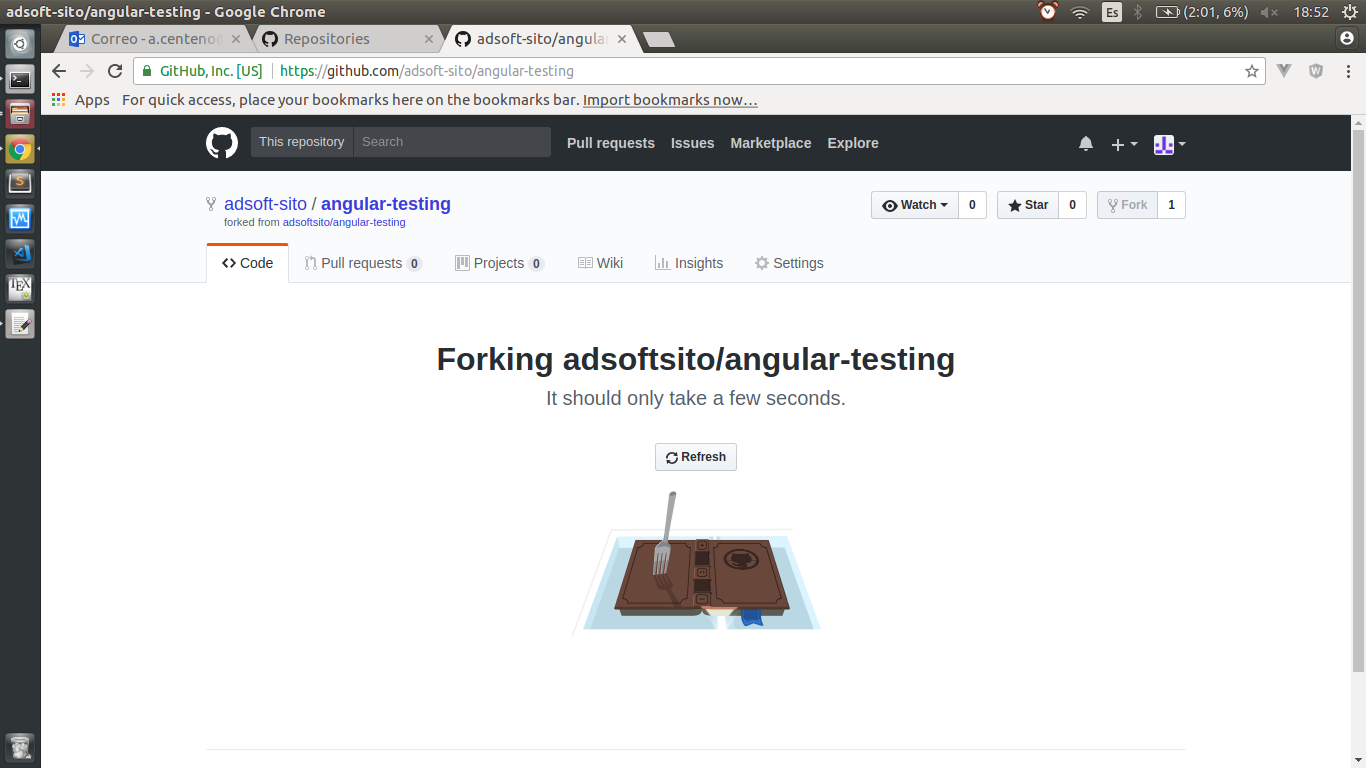
\includegraphics[width=0.9\textwidth]{forking.png}
\end{center}

\end{frame}

\begin{frame}\frametitle{} 


\begin{block}{clone your repo}
mkdir dev-testing \\
cd dev-testing	 \\
git clone -b develop https://github.com/your-own-repo/angular-testing.git \\
cd angular-testing \\
npm install \\
ng test   
\end{block}

\end{frame}


\begin{frame}\frametitle{} 


\begin{block}{currencies branch}
git branch \\
git branch currencies \\
git checkout currencies \\
git merge develop currencies \\
git branch 
\end{block}

\end{frame}


\begin{frame}\frametitle{} 

\begin{block}{create currencies feature}
cd src/app \\
mkdir currencies \\
cd currencies
\end{block}

\begin{block}{nano getCurrencies.spec.ts}
\lstspec
\end{block}

\begin{block}{nano getCurrencies.ts}
\lstts
\end{block}

\end{frame}




\begin{frame}\frametitle{} 


\begin{block}{push currencies}
cd .. \\
cd .. \\
pwd  \\
git add src/app/currencies \\
git commit -m "currencies feature" \\
git push -u origin currencies \\
\end{block}

\end{frame}


\begin{frame}\frametitle{} 

\begin{block}{Go to github}
\url{https://github.com/} \\

create a pull-request to develop branch in lider repo
\end{block}

\begin{center}
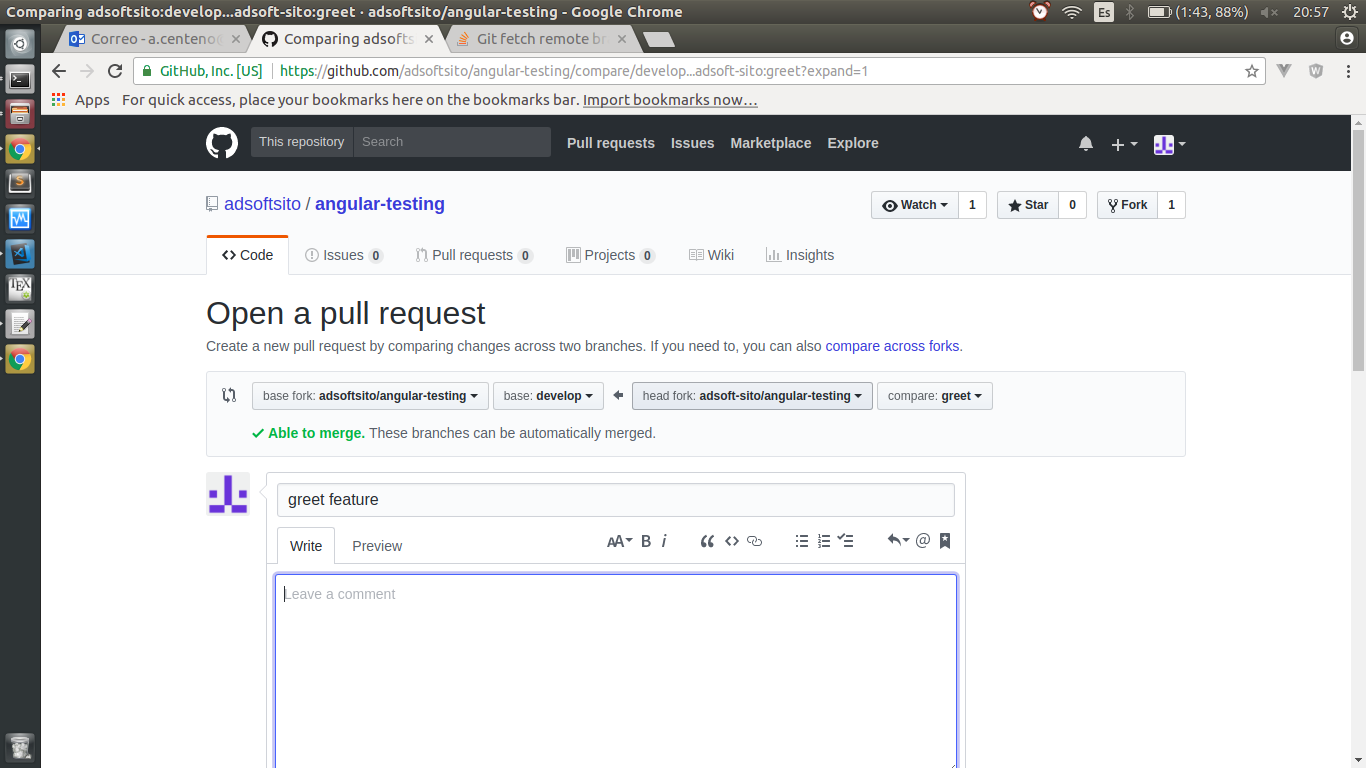
\includegraphics[width=0.9\textwidth]{pull-request.png}
\end{center}


\end{frame}

\end{document}
